\chapter{Arhitektura i dizajn sustava}
		
		\textbf{\textit{dio 1. revizije}}\\

		\textit{ Potrebno je opisati stil arhitekture te identificirati: podsustave, preslikavanje na radnu platformu, spremišta podataka, mrežne protokole, globalni upravljački tok i sklopovsko-programske zahtjeve. Po točkama razraditi i popratiti odgovarajućim skicama:}
	\begin{itemize}
		\item 	\textit{izbor arhitekture temeljem principa oblikovanja pokazanih na predavanjima (objasniti zašto ste baš odabrali takvu arhitekturu)}
		\item 	\textit{organizaciju sustava s najviše razine apstrakcije (npr. klijent-poslužitelj, baza podataka, datotečni sustav, grafičko sučelje)}
		\item 	\textit{organizaciju aplikacije (npr. slojevi frontend i backend, MVC arhitektura) }		
	\end{itemize}

	
		

		

		\pagebreak		
		\section{Baza podataka}
			
		Za naš sustav koristit ćemo relacijsku bazu podataka koja svojom strukturom olakšava modeliranje stvarnog svijeta. Gradivna jedinka baze je relacija, odnosno tablica koja je definirana svojim imenom i skupom atributa. Zadaća baze podataka je brza i jednostavna pohrana, izmjena i dohvat podataka za daljnju obradu.
		\newline
        Baza podataka ove aplikacije sastoji se od sljedećih entiteta: 
        \begin{itemize}
            \item Račun
            \item Klijent
            \item Tvrtka
            \item Vozilo
            \item Parkiralište
            \item Rezervacija
            \item Jednokratna
            \item Trajna
            \item Ponavljajuća
        \end{itemize}
        
		
			\subsection{Opis tablica}
			
			    \textbf{Račun} \newline
			    Entitet sadrži informacije o napravljenom računu u aplikaciji. Sadrži
			    atribute: ID, email, OIB, admin, lozinka. U vezi je \textit{One-To-Many} s entitetima Klijent i Tvrtka.
				
				\begin{longtabu} to \textwidth {|X[6, l]|X[6, l]|X[20, l]|}
					
					\hline \multicolumn{3}{|c|}{\textbf{Račun}}	 \\[3pt] \hline
					\endfirsthead
					
					\hline \multicolumn{3}{|c|}{\textbf{Račun}}	 \\[3pt] \hline
					\endhead
					
					\hline 
					\endlastfoot
					
					\cellcolor{LightGreen}ID & INT	&  jedinstveni identifikator računa \\ \hline
					email & VARCHAR &  e-mail adresa računa \\ \hline 
					OIB	& CHAR(11) &   oib osobe čiji je račun	\\ \hline 
					admin & BOOLEAN	&  	true ako je osoba administrator	\\ \hline 
					lozinka & VARCHAR	&  	hash lozinke	\\ \hline 
					
					
				\end{longtabu}
				
				\pagebreak
				\textbf{Klijent} \newline
			    Entitet sadrži informacije o klijentu koji koristi aplikaciju. Sadrži
			    atribute: ID, ime, prezime, broj kartice, računId. U vezi je \textit{One-To-Many} s entitetima Vozilo i Rezervacija, a s entitetom Račun je u vezi \textit{Many-To-One}.
				
				\begin{longtabu} to \textwidth {|X[6, l]|X[6, l]|X[20, l]|}
					
					\hline \multicolumn{3}{|c|}{\textbf{Klijent}}	 \\[3pt] \hline
					\endfirsthead
					
					\hline \multicolumn{3}{|c|}{\textbf{Klijent}}	 \\[3pt] \hline
					\endhead
					
					\hline 
					\endlastfoot
					
					\cellcolor{LightGreen}ID & INT	&  jedinstveni identifikator klijenta \\ \hline
					ime & VARCHAR &  ime klijenta \\ \hline 
					prezime & VARCHAR &  prezime klijenta \\ \hline 
					broj kartice & VARCHAR &  broj kartice klijenta \\ \hline 
					\cellcolor{LightBlue} računId	& VARCHAR &   jedinstveni identifikator računa (račun.ID)	\\ \hline 
					
					
				\end{longtabu}
				
				\textbf{Tvrtka} \newline
			    Entitet sadrži informacije o tvrtki koja želi prijaviti svoje parkilište u aplikaciji. Sadrži atribute: ID, naziv, adresa, računId. U vezi je \textit{One-To-Many} s entitetom Parkiralište, a s entitetom Račun je u vezi \textit{Many-To-One}.
				
				\begin{longtabu} to \textwidth {|X[6, l]|X[6, l]|X[20, l]|}
					
					\hline \multicolumn{3}{|c|}{\textbf{Tvrtka}}	 \\[3pt] \hline
					\endfirsthead
					
					\hline \multicolumn{3}{|c|}{\textbf{Tvrtka}}	 \\[3pt] \hline
					\endhead
					
					\hline 
					\endlastfoot
					
					\cellcolor{LightGreen}ID & INT	&  jedinstveni identifikator tvrtke \\ \hline
					naziv & VARCHAR &  naziv tvrtke \\ \hline 
					adresa & VARCHAR &  adresa sjedišta tvrtke \\ \hline 
					\cellcolor{LightBlue} računId	& VARCHAR &   jedinstveni identifikator računa (račun.ID)	\\ \hline 
					
					
				\end{longtabu}
				
				\textbf{Vozilo} \newline
			    Entitet sadrži informacije o vozilo kojeg je klijent prijavio. Sadrži
			    atribute: ID, registracija, naziv vozila, boja, i klijentId. U vezi je \textit{One-To-Many} s entitetom Rezervacija, a s entitetom Klijent je u vezi \textit{Many-To-One}.
				
				\begin{longtabu} to \textwidth {|X[6, l]|X[6, l]|X[20, l]|}
					
					\hline \multicolumn{3}{|c|}{\textbf{Vozilo}}	 \\[3pt] \hline
					\endfirsthead
					
					\hline \multicolumn{3}{|c|}{\textbf{Vozilo}}	 \\[3pt] \hline
					\endhead
					
					\hline 
					\endlastfoot
					
					\cellcolor{LightGreen}ID & INT	&  jedinstveni identifikator vozila \\ \hline
					registracija & VARCHAR &  broj registracije vozila \\ \hline 
					naziv vozila & VARCHAR &  naziv vozila koje dodjeluje klijent \\ \hline 
					boja & VARCHAR &  boja vozila koju dodjeluje klijent \\ \hline 
					\cellcolor{LightBlue} klijentId	& VARCHAR &   jedinstveni identifikator klijenta (klijent.ID)	\\ \hline 
					
				\end{longtabu}
				
				\pagebreak
				\textbf{Parkiralište} \newline
			    Entitet sadrži informacije o parkiralištu neke tvrtke koje se nudi klijentima. Sadrži
			    atribute: ID, naziv, broj mjesta, broj invalidskih mjesta, tip prakirališta, koordinate, cijena jednokratne, cijena ponavljajuće, cijena trajne i tvrtkaId. U vezi je \textit{One-To-Many} s entitetom Rezervacija, a s entitetom Tvrtka je u vezi \textit{Many-To-One}.
				
				\begin{longtabu} to \textwidth {|X[6, l]|X[6, l]|X[20, l]|}
					
					\hline \multicolumn{3}{|c|}{\textbf{Parkiralište}}	 \\[3pt] \hline
					\endfirsthead
					
					\hline \multicolumn{3}{|c|}{\textbf{Parkiralište}}	 \\[3pt] \hline
					\endhead
					
					\hline 
					\endlastfoot
					
					\cellcolor{LightGreen}ID & INT	&  jedinstveni identifikator parkirališta \\ \hline
					naziv & VARCHAR &  naziv parkirališta \\ \hline 
					broj mjesta & INT &  broj mjesta koje parkiralište nudi \\ \hline 
					broj invalidskih mjesta & INT &  broj invalidskih mjesta koje ima parkiralište \\ \hline tip parkirališta & VARCHAR &  tip parkirališta (otvoreno, zatvoreno) \\ \hline 
					koordinate & VARCHAR &  zemljopisna dužina i širina parkirališta \\ \hline 
					cijena jednokratne & INT &  cijena sata za jednokratnu rezervaciju parkirališta \\ \hline 
					cijena ponavljajuće & INT &  cijena sata za ponavljajuću rezervaciju parkirališta \\ \hline
					cijena trajne & INT &  cijena trajne rezervacije parkirališta \\ \hline
					\cellcolor{LightBlue} tvrtkaId	& VARCHAR &   jedinstveni identifikator tvrtke (tvrka.ID)	\\ \hline 
					
					
				\end{longtabu}
				
				
				\textbf{Rezervacija} \newline
			    Entitet sadrži informacije o stvorenoj rezervaciji u aplikaciji. Ima
			    atribute: ID, klijentId, parkirališteId, voziloId. U vezi je \textit{One-To-Many} s entitetima Jednokratna, Ponavljajuća i Trajna. S entitetima Klijent, Parkiralište i Vozilo je u vezi \textit{Many-To-One}.
				
				\begin{longtabu} to \textwidth {|X[6, l]|X[6, l]|X[20, l]|}
					
					\hline \multicolumn{3}{|c|}{\textbf{Rezervacija}}	 \\[3pt] \hline
					\endfirsthead
					
					\hline \multicolumn{3}{|c|}{\textbf{Rezervacija}}	 \\[3pt] \hline
					\endhead
					
					\hline 
					\endlastfoot
					
					\cellcolor{LightGreen}ID & INT	&  jedinstveni identifikator rezervacije \\ \hline
					\cellcolor{LightBlue} klijentId	& VARCHAR &   jedinstveni identifikator klijenta (klijent.ID)	\\ \hline
					\cellcolor{LightBlue} parkirališteId	& VARCHAR &   jedinstveni identifikator prakirališta (parkiralište.ID)	\\ \hline
					\cellcolor{LightBlue} voziloId	& VARCHAR &   jedinstveni identifikator vozila (vozilo.ID)	\\ \hline
					
				\end{longtabu}
				
				\pagebreak
				\textbf{Jednokratna} \newline
			    Entitet sadrži informacije o jednokratnoj rezervaciji stvorenoj u aplikaciji. Ima
			    atribute: ID, vrijeme početak, vrijeme kraj, rezervaijaId. U vezi je \textit{Many-To-One} s entitetom Rezervacija.
			    
				\begin{longtabu} to \textwidth {|X[6, l]|X[6, l]|X[20, l]|}
					
					\hline \multicolumn{3}{|c|}{\textbf{Jednokratna}}	 \\[3pt] \hline
					\endfirsthead
					
					\hline \multicolumn{3}{|c|}{\textbf{Jednokratna}}	 \\[3pt] \hline
					\endhead
					
					\hline 
					\endlastfoot
					
					\cellcolor{LightGreen}ID & INT	&  jedinstveni identifikator jednokratne rezervacije \\ \hline
					vrijeme početak & TIMESTAMP &  vrijeme početka rezervacije \\ \hline  
					vrijeme kraj & TIMESTAMP &  vrijeme kraja rezervacije \\ \hline 
					\cellcolor{LightBlue} rezervacijaId	& VARCHAR &   jedinstveni identifikator rezervacije (rezervacija.ID)	\\ \hline
					
				\end{longtabu}
				
				\textbf{Trajna} \newline
			    Entitet sadrži informacije o trajnoj rezervaciji stvorenoj u aplikaciji. Ima
			    atribute: ID, vrijeme početak, vrijeme kraj, rezervaijaId. U vezi je \textit{Many-To-One} s entitetom Rezervacija.
				
				\begin{longtabu} to \textwidth {|X[6, l]|X[6, l]|X[20, l]|}
					
					\hline \multicolumn{3}{|c|}{\textbf{Trajna}}	 \\[3pt] \hline
					\endfirsthead
					
					\hline \multicolumn{3}{|c|}{\textbf{Trajna}}	 \\[3pt] \hline
					\endhead
					
					\hline 
					\endlastfoot
					
					\cellcolor{LightGreen}ID & INT	&  jedinstveni identifikator trajne rezervacije \\ \hline
					vrijeme početak & TIMESTAMP &  vrijeme početka rezervacije \\ \hline  
					vrijeme kraj & TIMESTAMP &  vrijeme kraja rezervacije \\ \hline 
					\cellcolor{LightBlue} rezervacijaId	& VARCHAR &   jedinstveni identifikator rezervacije (rezervacija.ID)	\\ \hline
					
				\end{longtabu}
				
				\pagebreak
				\textbf{Ponavljajuća} \newline
			    Entitet sadrži informacije o ponavljaućoj rezervaciji stvorenoj u aplikaciji. Ima
			    atribute: ID, datum rezervacije, datum kraja rezervcije, dani ponavljanja, vrijeme početak, vrijeme kraj i rezervaijaId. U vezi je \textit{Many-To-One} s entitetom Rezervacija.
				
				\begin{longtabu} to \textwidth {|X[6, l]|X[6, l]|X[20, l]|}
					
					\hline \multicolumn{3}{|c|}{\textbf{Ponavljajuća}}	 \\[3pt] \hline
					\endfirsthead
					
					\hline \multicolumn{3}{|c|}{\textbf{Ponavljajuća}}	 \\[3pt] \hline
					\endhead
					
					\hline 
					\endlastfoot
					
					\cellcolor{LightGreen}ID & INT	&  jedinstveni identifikator ponavljajuće rezervacije \\ \hline
					datum rezervacije & DATE &  datum početka rezervacije \\ \hline
					datum kraja rezervacije & DATE &  datum kraja rezervacije \\ \hline
					dani ponavljanja & INT &  dani ponavljanje rezervacije (pon=1, uto=2, ...) \\ \hline
					vrijeme početak & TIME &  vrijeme početka rezervacije \\ \hline  
					vrijeme kraj & TIME &  vrijeme kraja rezervacije \\ \hline 
					\cellcolor{LightBlue} rezervacijaId	& VARCHAR &   jedinstveni identifikator rezervacije (rezervacija.ID)	\\ \hline
					
				\end{longtabu}
				
				
			
			\pagebreak
			\subsection{Dijagram baze podataka}
                \begin{figure}[H]
                	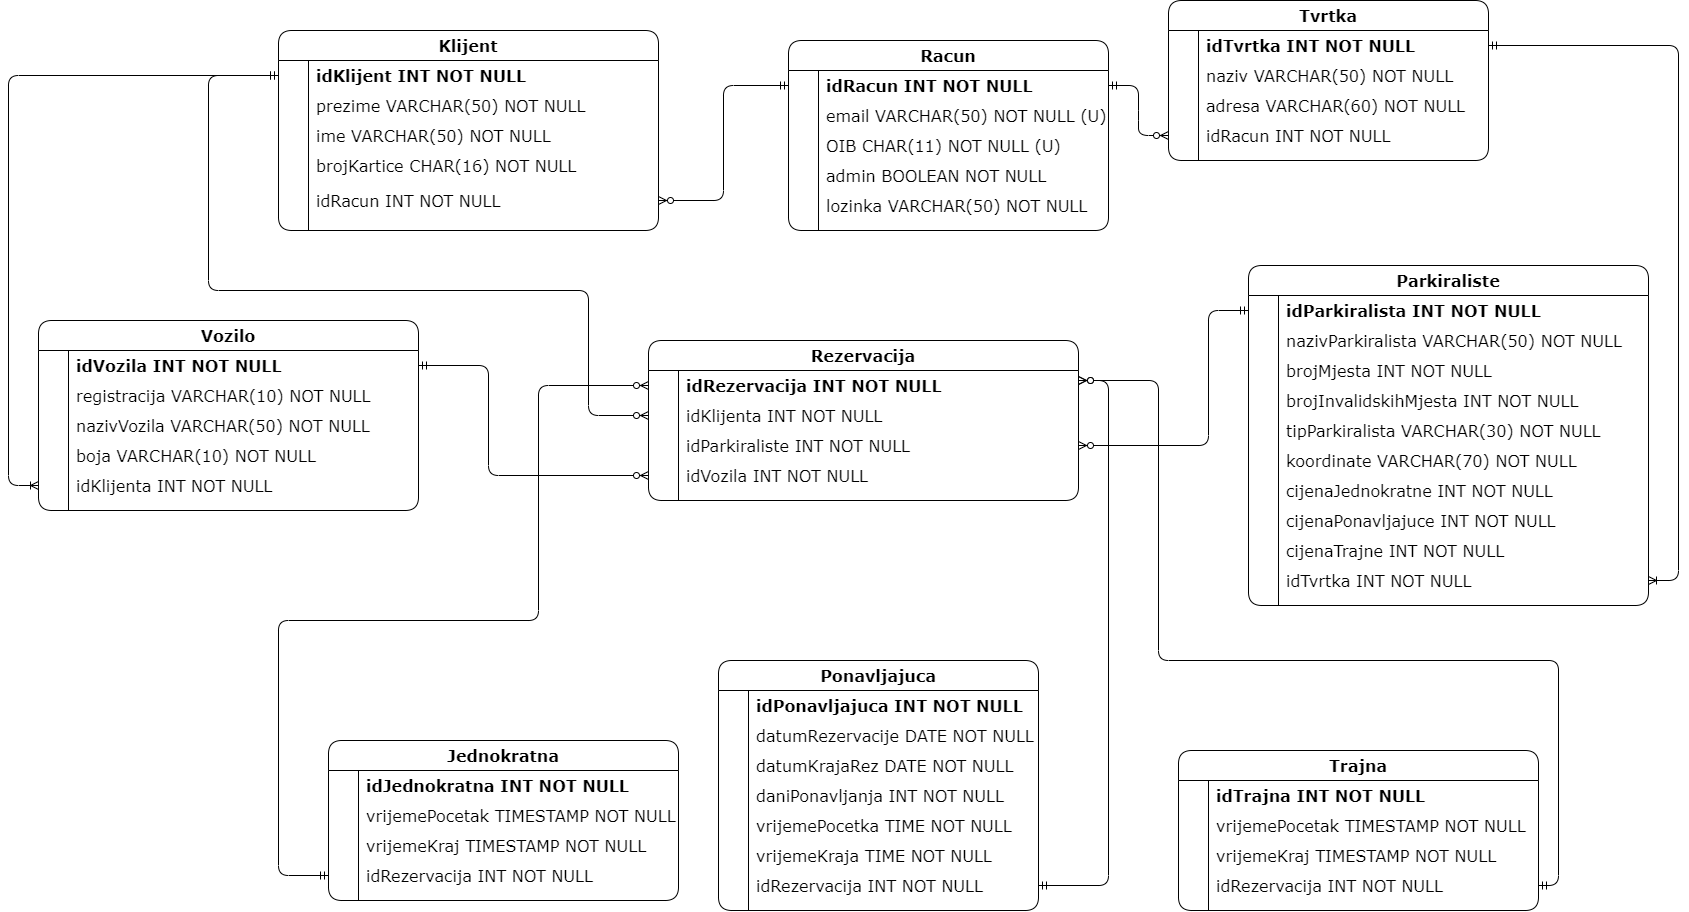
\includegraphics[width=1\linewidth]{dijagrami/ERModel.png} %veličina u odnosu na širinu linije
                	\caption{Prikaz funkcionalnosti vezanih za korisničke podatke}
                	\label{fig:promjene2} %label mora biti drugaciji za svaku sliku
                \end{figure}
			
			\eject
			
			
		\section{Dijagram razreda}
		
			\textit{Potrebno je priložiti dijagram razreda s pripadajućim opisom. Zbog preglednosti je moguće dijagram razlomiti na više njih, ali moraju biti grupirani prema sličnim razinama apstrakcije i srodnim funkcionalnostima.}\\
			
			\textbf{\textit{dio 1. revizije}}\\
			
			\textit{Prilikom prve predaje projekta, potrebno je priložiti potpuno razrađen dijagram razreda vezan uz \textbf{generičku funkcionalnost} sustava. Ostale funkcionalnosti trebaju biti idejno razrađene u dijagramu sa sljedećim komponentama: nazivi razreda, nazivi metoda i vrste pristupa metodama (npr. javni, zaštićeni), nazivi atributa razreda, veze i odnosi između razreda.}\\
			
			\textbf{\textit{dio 2. revizije}}\\			
			
			\textit{Prilikom druge predaje projekta dijagram razreda i opisi moraju odgovarati stvarnom stanju implementacije}
			
			
			
			\eject
		
		\section{Dijagram stanja}
			
			
			\textbf{\textit{dio 2. revizije}}\\
			
			\textit{Potrebno je priložiti dijagram stanja i opisati ga. Dovoljan je jedan dijagram stanja koji prikazuje \textbf{značajan dio funkcionalnosti} sustava. Na primjer, stanja korisničkog sučelja i tijek korištenja neke ključne funkcionalnosti jesu značajan dio sustava, a registracija i prijava nisu. }
			
			
			\eject 
		
		\section{Dijagram aktivnosti}
			
			\textbf{\textit{dio 2. revizije}}\\
			
			 \textit{Potrebno je priložiti dijagram aktivnosti s pripadajućim opisom. Dijagram aktivnosti treba prikazivati značajan dio sustava.}
			
			\eject
		\section{Dijagram komponenti}
		
			\textbf{\textit{dio 2. revizije}}\\
		
			 \textit{Potrebno je priložiti dijagram komponenti s pripadajućim opisom. Dijagram komponenti treba prikazivati strukturu cijele aplikacije.}